% =====================================================================
% When Errors Become Narratives: A Longitudinal Taxonomy of Silent
% Failures in a Production LLM Agent Runtime
%
% ISSRE 2026 Industry Track -- CONSERVATIVE 6-page trim (incl. refs).
% IEEE Computer Society conference format (IEEEtran).
% Build: pdflatex issre_6page_trimmed.tex  (twice for cross-refs).
%
% This is the PRE-TRIMMED variant of issre_6page.tex: the "Trim
% priorities" order is already applied (Sec.II compressed; D2-D4 to
% one sentence each; Sec.VI as a bare list; secondary prose tightened)
% to land at/under 6 pages WITHOUT touching the load-bearing content:
% Sec.III method, the 0%/87% scorecard, Sec.VIII threats, the GenAI
% disclosure, Table 1, D1 + Fig.1, the reserved-file incident, and every
% frozen number stay intact.
%
% Numbers FROZEN at study cutoff 2026-06-11 (matches arXiv:2606.14589).
% AFTER compiling: confirm <= 6 pages incl. refs (over = desk reject).
% If still slightly over, cut the 9-hour-outage clause in Sec.IV-E and
% the LLM-judge tangent in Sec.V (discovery). If UNDER 6 pages with
% room, restore detail from issre_6page.tex.
% Author: Wei Wu <wuweinanonuaa@gmail.com>, Independent Researcher.
% =====================================================================
\documentclass[conference]{IEEEtran}
\IEEEoverridecommandlockouts

\usepackage[T1]{fontenc}
\usepackage[utf8]{inputenc}
\usepackage{cite}
\usepackage{amsmath,amssymb}
\usepackage{graphicx}
\usepackage{booktabs}
\usepackage{array}
\usepackage{xcolor}
\usepackage{tikz}
\usetikzlibrary{arrows.meta,positioning,calc}
\usepackage[hidelinks]{hyperref}

\newcommand{\failplausible}{\emph{fail-plausible}}

\tikzset{
  box/.style={draw, rounded corners=2pt, align=center, font=\scriptsize,
              inner sep=3pt, text width=6.6cm, minimum height=12pt},
  bad/.style={box, fill=red!8, draw=red!60!black},
  amp/.style={box, fill=orange!12, draw=orange!70!black},
  con/.style={box, fill=yellow!18, draw=yellow!55!black},
  good/.style={box, fill=green!10, draw=green!50!black},
  flow/.style={-{Stealth[length=2mm]}, thick},
}

\begin{document}

\title{When Errors Become Narratives: A Longitudinal\\Taxonomy of Silent
Failures in a Production LLM Agent Runtime}

\author{\IEEEauthorblockN{Wei Wu}
\IEEEauthorblockA{Independent Researcher\\
wuweinanonuaa@gmail.com}}

\maketitle

\begin{abstract}
LLM agent systems increasingly run as long-running autonomous runtimes:
scheduling jobs, calling tools, maintaining memory, messaging humans. We
present an eight-week longitudinal study of silent failures in one
production personal-assistant runtime ($\sim$40 scheduled jobs, 8 LLM
providers, a tool-governance proxy, a knowledge-base memory plane;
4{,}286 unit tests, 827 governance checks). We documented 22 incidents
with full postmortems; one meta-pattern---an error signal that never
reaches a human in actionable form---recurred at least 28 times. We
derive a five-class mechanism taxonomy: (A)~environment quirks,
(B)~design-assumption mismatches, (C)~error swallowing, (D)~chained
hallucination, (E)~operational omission. Class~D is LLM-specific and most
dangerous: the model transforms errors into fluent, false narrative---we
name this \failplausible. Three findings challenge assumptions:
$\sim$70\% of failures surfaced through human user-view observation, not
tests; audits showed 0\% prevention but 87\% regression-blocking; latency
(13 hours to 60 days) tracks mechanism, not code complexity.
\end{abstract}

\begin{IEEEkeywords}
software reliability; LLM agent systems; silent failures; fault taxonomy
\end{IEEEkeywords}

\section{Introduction}
The reliability literature has long known that the most damaging failures
are not crashes. \emph{Gray failures}~\cite{huang2017gray} degrade cloud
systems while their failure detectors report health; \emph{fail-slow}
hardware~\cite{gunawi2018failslow} throttles for hours before anyone
suspects the disk. The defining property of both is \textbf{differential
observability}: the application suffers, but the observer designed to
notice does not.

LLM agent systems inherit this problem class---and add a new one. An agent
runtime is a generator of fluent language; when an upstream error leaks
into its context window, its failure mode is not silence but
\emph{plausible speech}. In one incident (\S\ref{sec:taxonomy}), an
HTTP~400 error page was captured into a cache by a logging bug, and the
downstream LLM---seeing error strings where signals should be---confidently
fabricated an industry analysis about a ``Hugging Face platform crisis''
and pushed it to the user as a routine digest. No detector fired; every
test was green. The error had not disappeared; it had been
\emph{narrated}. We call this \failplausible: the system transforms an
internal error into coherent, contextually appropriate, false output.
Fail-plausible is to LLM agents what gray failure was to cloud
infrastructure---the dominant, hardest-to-see class---but strictly worse:
gray failure starves the detector of signal; fail-plausible feeds the
human a counterfeit one.

This paper reports what eight weeks of documented production incidents
taught us, in five contributions: (1)~a \textbf{mechanism-oriented
taxonomy} (\S\ref{sec:taxonomy}) of five silent-failure classes from 22
documented incidents, classified by mechanism rather than location,
because the same mechanism recurs across components and a mechanism-level
defense immunizes a class rather than a file; (2)~the
\textbf{fail-plausible class} (\S\ref{sec:classd}), four incidents in
which LLMs converted polluted context into confident
fabrications---fabricated releases, platform crises, host-OS remediation
instructions; (3)~\textbf{quantified findings} (\S\ref{sec:findings}):
latency 13 hours--60 days, $\sim$70\% human user-view discovery (tests
$\approx$0\%), a trigger/amplifier/concealer structure, and one
meta-pattern manifesting $\geq$28 times---silent failure is a \emph{bug
class}; (4)~an \textbf{audited defense framework}
(\S\ref{sec:defense})---0\% ex-ante prevention, 87\% ex-post
regression-blocking: \emph{audit is a regression engine, not a prediction
engine}; and (5)~a \textbf{complexity argument}
(\S\ref{sec:discussion}): the longest failures lived in \emph{seams}, not
complex components, motivating a ``Sunset Law'' that ranks retiring
complexity over adding protection. The study is a \textbf{longitudinal
single-case study} (\S\ref{sec:method})---the complement to horizontal
studies that sample failures from benchmark traces~\cite{cemri2025mast} or
provider incident databases~\cite{ranganathan2025inference}, which cannot
see the longitudinal texture (multi-week latency, discovery channels,
defense evolution) that only a continuously operating, fully-postmortemed
system exposes.

\section{Background and Related Work}
\textbf{Silent failures in distributed systems.} Gray failure named the
mode behind most cloud incidents---components degrade while detectors
report health (differential observability)~\cite{huang2017gray}; fail-slow
at scale documented 101--114 hardware-fault reports with cascading root
causes and multi-hundred-hour diagnosis~\cite{gunawi2018failslow}. We are
downstream of this tradition but at the LLM-agent layer, with every
incident \emph{silent} by selection; Classes~C and~E are familiar to that
readership, Class~D is not.

\textbf{LLM agent failures.} MAST is the first grounded multi-agent LLM
failure taxonomy---14 modes from 1{,}600+ benchmark traces, $\kappa$=0.88%
~\cite{cemri2025mast}---but its unit is the task trace, where failures show
as non-completion; our unit is the production incident that failed no task
and kept detectors green. A study of 156 inference
incidents~\cite{ranganathan2025inference} shares our production grounding
but at the (loud) inference-service layer. Ezell et al.\ argue for
structured agent incident analysis~\cite{ezell2025incident}; our corpus is
an existence proof that adds the requirement to record \emph{how long a
failure was silent and who noticed}. Work on agentic exception
handling~\cite{zhou2025shielda}, incident response~\cite{xiao2026air}, and
MCP fault taxonomies~\cite{taraghi2026mcp,owotogbe2026mcpruntime} does not
target the silent/fail-plausible class.

\textbf{Hallucination and practice.} Hallucination is usually a
\emph{model} property~\cite{huang2023hallucination}; our Class~D reframes
it as a \emph{systems} property---in 4/4 incidents the model completed
fluently as trained, and the failure was that the system delivered
polluted context, so the defense is system-side. SRE codified engineering
(not remembering) operational knowledge~\cite{beyer2016sre}, which our
convergence engine applies to declared state; chaos engineering
established fault injection~\cite{basiri2016chaos}, which we lift to
\emph{sabotage validation} of the guards (an unvalidated detector is
indistinguishable from a vacuous one). Large-scale incident
studies~\cite{ghosh2022fight} set the corpus/root-cause/automation-gap
template we instantiate; the variable we add is that the system
\emph{speaks}, changing what failure looks like (\S\ref{sec:classd}) and
what detection requires (\S\ref{sec:discovery}).

\section{Research Method and System Context}\label{sec:method}
We frame this as a \textbf{longitudinal single-case study} in the sense of
Runeson and H\"ost~\cite{runeson2009case}, so ``n=1'' is a deliberate
design with an explicit generalization argument.

\textbf{Method rationale.} Case study fits for three reasons grounded in
the phenomenon: silent failures are \emph{not reproducible on demand}
(they manifest only in a continuously operating system whose indicators
stay green, precluding controlled experiments and benchmark-trace
sampling); the variables of interest---silence latency, discovery channel,
defense evolution---only exist over real operational time; and the unit is
an \emph{operating system in context}. The case is \emph{revelatory}
(public access to production fail-plausible fabrication with complete
causal-chain postmortems) and \emph{longitudinal} (eight weeks in which
failures and defenses co-evolve).

\textbf{The case.} The subject (public repository
\texttt{openclaw-model-bridge}) is two-layer middleware connecting
self-hosted and commercial LLMs to OpenClaw, an open-source personal-agent
framework, in continuous production on one macOS host since early March
2026. Three planes: a \textbf{control plane} (tool-governance proxy with a
hard tool cap, schema repair, alert stripping; a declarative engine of 90
invariants / 827 checks / 23 meta-rules / 14 mechanized scanners with a
daily audit; SLO monitoring; circuit breakers; a convergence engine
synchronizing declared to runtime state); a \textbf{capability plane} (an
adapter routing across 8 providers with capability-scored fallback
chains); and a \textbf{memory plane} (a $\sim$1{,}100-note local-embedding
RAG index, media index, conversation harvesting, daily LLM synthesis jobs
that push insights to the user). Scale at the cutoff (2026-06-11):
$\sim$40 scheduled jobs across two cron schedulers; 8 providers; 3
supervised services; 4{,}286 unit tests in 121 suites; 22 published
postmortems. One human operator and one AI engineering collaborator
develop and operate the system, whose runtime is powered by \emph{separate}
models---also a data point on AI-assisted operation of an AI system
(\S\ref{sec:discussion}).

\textbf{Unit and corpus.} The unit is the \emph{silent-failure
incident}---an event that (a)~reached production, (b)~had a silent phase
with all automated indicators green, and (c)~closed with a complete
postmortem; the embedded sub-unit is the \emph{mechanism}. The
single-case-with-embedded-units design (case~=~the runtime; units~=~22
incidents $\to$ $\geq$28 mechanism manifestations) licenses within-case
cross-incident comparison with context fixed. The corpus is the
\textbf{complete population} of qualifying incidents in the window
(2026-04-09 to 2026-06-02), not a sample.

\textbf{Data collection.} A \textbf{fixed postmortem protocol}, adopted
after the second incident and applied retroactively to the first two,
mandates before any fix: a causal-chain diagram; a three-layer root cause
(\emph{trigger / amplifier / concealer}); a timeline; a ``why now''
condition-combination analysis; and an entry feeding the governance
ontology. This triangulates across runtime logs, the OS audit log, version
control, test/governance results, and the operator's notes---each incident
corroborated by $\geq$2 independent sources before root cause is recorded.

\textbf{Analysis and generalization.} Classification used \textbf{constant
comparison}; two consecutive non-matches forced a new class. We classify
by mechanism because a location taxonomy had no defensive value whereas a
mechanism-level defense immunizes a class; the scheme stabilized over the
final 9 incidents (saturation). The classes are \emph{load-bearing}: each
drives a scanner with objective findings, so a misclassification is
falsifiable. We claim \textbf{analytical generalization} (to theory), not
statistical: the five classes, the trigger/amplifier/concealer structure,
the latency~$\propto$~observational-distance relationship, the point
fix~$\to$~meta-rule~$\to$~scanner maturation, and audit-as-regression-engine
are mechanism claims with ancestry in prior literature (A,~C,~E) or in a
property common to LLM runtimes (D). The frequencies and shares are
descriptive statistics of this case; the $\sim$70\% user-view share is an
\textbf{existence proof}, not a constant.

\section{A Taxonomy of Silent Failures}\label{sec:taxonomy}
Table~\ref{tab:taxonomy} summarizes the five classes.

\begin{table*}[t]
\centering
\caption{Five classes over 22 incidents (+ sub-events).}
\label{tab:taxonomy}
\footnotesize
\begin{tabular}{@{}p{2.4cm}p{5.2cm}cp{1.6cm}p{4.4cm}@{}}
\toprule
\textbf{Class} & \textbf{Mechanism} & \textbf{Inc.} & \textbf{Silence} & \textbf{Defining property}\\
\midrule
A --- Environment/platform quirk & Logic correct; runtime environment's implicit behavior defeats it & 1 (+6) & hrs--wks & dev green; only target OS/client reveals\\
B --- Design-assumption mismatch & Code assumes a topology/contract/input shape reality violates & 4 & days & tests cover the assumption, not reality\\
C --- Error swallowing \& dilution & Error occurs, is eaten or stripped of cause across layers & 5 & hrs--days & the alert carries no usable information\\
D --- Chained hallucination & LLM converts polluted context into confident false output & 4 & hrs--days & \textbf{fail-plausible}: user receives counterfeit health\\
E --- Operational omission \& forensic blind spot & A deploy/registration step is skipped, or the forensic tool itself is blocked and reads ``normal'' & 8 & days--\textbf{60d} & declared $\neq$ runtime state; instruments lie\\
\bottomrule
\end{tabular}
\end{table*}

\subsection{Class A --- Environment and platform quirks}
\emph{The logic is right; the environment's implicit behavior is not what
anyone assumed.} The dev environment (Linux, root, GNU userland, bash~5)
is systematically more permissive than the production target (macOS, bash
3.2, BSD userland, sandboxed cron). Sub-events: bash 3.2 not propagating
ERR traps into functions without \texttt{set~-E}, disarming a watchdog
self-alarm; BSD awk aborting on invalid UTF-8 which---with
\texttt{set~-e}---killed the \emph{monitoring} script for 7 days; missing
GNU \texttt{timeout} turning a defensive wrapper into a universal ``tool
unavailable''; and a messaging client folding long messages at an
undocumented $\sim$4{,}000-char threshold. The signature is \textbf{green
dev, silent prod}; the defense is mechanized---a cross-OS quirk scanner
encodes six known patterns, and a meta-rule requires framework fixes to be
validated \emph{on the target environment}, after a dev-only fix shipped
broken twice in one day.

\subsection{Class B --- Design-assumption mismatches}
\emph{Code internally consistent with an assumption; production violates
it.} A metadata-resolution function shipped three path candidates for a
registry file, all missing its production location; the component fell
back silently to an unfiltered mode for \textbf{five days} while a
companion feature silently never ran---unit tests green throughout because
their fixtures embodied the same wrong assumption. Likewise, an LLM-output
parser indexed lines positionally; the model occasionally omits a line
(instruction-following is a distribution, not a contract), shifting every
field one slot. \textbf{Any positional parse of LLM output is a latent
Class~B failure}---frozen into a meta-rule (parsers must be key-based) and
a scanner. Signature: \emph{tests mirror the assumption, not the caller.}

\subsection{Class C --- Error swallowing and dilution}
\emph{The error happens and is reported---into a void.} \textbf{Swallowing:}
a summary counted only \texttt{status=="fail"}, so invariants raising an
exception vanished and the audit printed ``all invariants hold'' over dead
checks; in a later echo, 67 checks (across 21 invariants) silently ran
\texttt{exec("")} for months, found only when a new sabotage refused to
fail. \textbf{Dilution:} an ``HTTP~502'' digest failure hid its true
cause (a fallback provider's quota exhausted after the primary's breaker
opened) across three hops that each stripped cause, so the alert reaching
the human carried zero actionable bits; in agent systems the ``client'' of
an error is often another LLM prompt, one step from Class~D input.
\textbf{Amplified swallowing:} a batch tool injected an env-var read into 8
scripts without the import---a \texttt{NameError} in all 8, caught by a
fail-open guard that skipped the new validation in all 8 while every test
passed. Automation is a bug amplifier.

\subsection{Class D --- Chained hallucination (fail-plausible)}\label{sec:classd}
\emph{The most dangerous class, without precedent in the gray-failure
literature.} The error is not suppressed; it is \textbf{transformed}.

\emph{D1 --- The fabricated platform crisis.} A nightly synthesis job
collects signals from $\sim$290 notes via map-reduce LLM calls. A Unicode
surrogate made the JSON serializer raise mid-write, truncating the request
body into a 400; and the chain turns: the map step logged diagnostics to
\textbf{stdout}, the caller captured stdout by command substitution as the
\emph{signal payload}, and the cache filled with HTTP-error strings. The
reduce-step LLM, prompted for cross-domain signals, composed a confident
analysis of a ``Hugging Face platform crisis''---platform trouble being
the most probable narrative shell for error-code vocabulary---pushed to
the user as a routine digest. Every component succeeded; the pipeline
laundered an encoding bug into industry analysis (Fig.~\ref{fig:d1}). The
structural fix was four layers deep, but the load-bearing one was a single
stderr redirection: \textbf{one redirection operator severed the entire
hallucination chain.}

\begin{figure}[t]
\centering
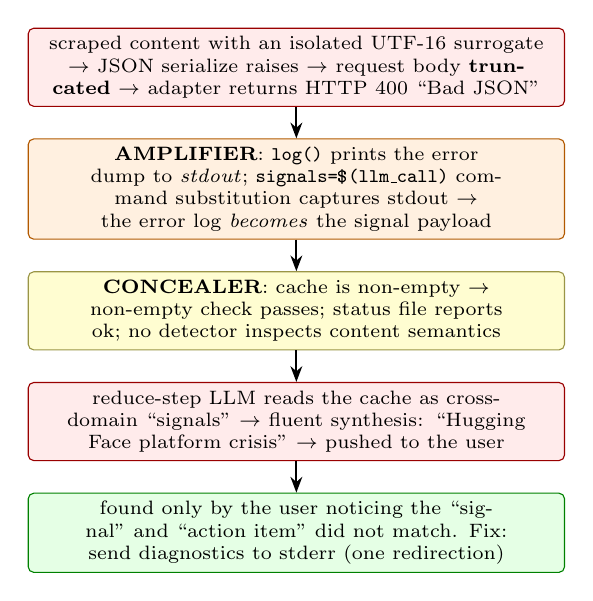
\begin{tikzpicture}[node distance=4mm]
\node[bad] (a) {scraped content with an isolated UTF-16 surrogate $\to$ JSON serialize raises $\to$ request body \textbf{truncated} $\to$ adapter returns HTTP 400 ``Bad JSON''};
\node[amp, below=of a] (b) {\textbf{AMPLIFIER}: \texttt{log()} prints the error dump to \emph{stdout}; \texttt{signals=\$(llm\_call)} command substitution captures stdout $\to$ the error log \emph{becomes} the signal payload};
\node[con, below=of b] (c) {\textbf{CONCEALER}: cache is non-empty $\to$ non-empty check passes; status file reports ok; no detector inspects content semantics};
\node[bad, below=of c] (d) {reduce-step LLM reads the cache as cross-domain ``signals'' $\to$ fluent synthesis: ``Hugging Face platform crisis'' $\to$ pushed to the user};
\node[good, below=of d] (e) {found only by the user noticing the ``signal'' and ``action item'' did not match. Fix: send diagnostics to stderr (one redirection)};
\draw[flow] (a)--(b); \draw[flow] (b)--(c); \draw[flow] (c)--(d); \draw[flow] (d)--(e);
\end{tikzpicture}
\caption{The D1 pollution chain: one malformed byte to a fabricated
industry analysis. Every component behaves as designed. (Refine as a
camera-ready vector figure.)}
\label{fig:d1}
\end{figure}

\emph{D2 --- The fabricated remediation.} A watchdog alert persisted into
chat history as an assistant message led the model, 36 minutes later, to
fabricate that it had ``received the system alert follow-up task'' and
instruct the user to grant Full Disk Access to a cron binary---off-topic
and ungrounded, because alert traffic and conversation are different
speech acts that must not share a context window.

\emph{D3 --- The fabricated success.} A weekly-review job whose LLM call
failed fell back to a line-filter emitting leftover container headings as
review content while writing a success flag unconditionally---\textbf{a
fallback that manufactures plausible-shaped output is a hallucination
implemented in shell.}

\emph{D4 --- The fabricated release.} An evening digest, given the day's
papers as enrichment, inferred the project ``must have shipped'' and
announced a release of an internal version number that exists only in the
changelog---\emph{true but unlabeled} context is fabrication fuel.

The common structure is a \textbf{pollution chain}: a Class~A/B/C failure
deposits non-signal content where a downstream LLM expects signal; the LLM
completes fluently, and the output inherits the \emph{form} of health with
the \emph{content} of failure. Defense is system-side context hygiene at
every link: stderr discipline; alert stripping before context assembly;
provenance/credibility labeling; and a six-level cumulative ladder of
anti-fabrication prompt guards, shared as one imported module across all
nine LLM-calling jobs. Prompt guards are the \emph{last} layer, behind
hygiene and provenance (\S\ref{sec:maturation}).

\subsection{Class E --- Operational omission and forensic blind spots}
\emph{The code is right; an operational step never happened---or the
diagnostic instrument itself is compromised.} The largest class (8) with
the longest silences. \emph{Omission:} a fully implemented, tested,
registered, deployed daily job never ran because the final step (writing
the crontab line) was a human memory item, hidden by three small bugs (a
preflight grepping only one of two drift strings; a crontab helper
ignoring its exit code and comparing counts with ``$<$''; no log on
absence). This drove the system's largest correction: \textbf{declared
state must converge to runtime state via machine, not memory}---a
convergence engine diffing declarations against observed
crontab/launchd/provider state on every audit, with staged escalation.
\emph{The reserved-file incident:} the agent wrote ``task complete'' notes
into a file named \texttt{HEARTBEAT.md}---to it a scratch filename, to the
runtime a \emph{reserved control file} whose non-empty content activates a
heartbeat protocol that makes the model reply with a bare acknowledgment
token, which the gateway then strips from outbound messages. For 13 hours
every user message returned a reply stripped to nothing in
transit---\textbf{total silence, every component working exactly as
designed.} \emph{Forensic blind spots:} the longest silence---\textbf{60
days}---was an external-SSD backup failing with EPERM; six hypotheses were
each falsified by data over weeks, and the breakthrough came only from the
OS audit log (macOS sandbox denials: cron-derived processes lack Full Disk
Access). The deeper finding: during those weeks the \emph{forensic
collectors themselves} were silently denied and returned empty output,
recorded as ``normal/empty.'' \textbf{An instrument that cannot
distinguish ``nothing there'' from ``I was not allowed to look''
manufactures false reassurance.} A 9-hour gateway outage whose three
independent alarms each failed yielded the rule that \textbf{an alert path
must not depend on the failing subject}.

\section{Cross-Cutting Findings}\label{sec:findings}
\textbf{Latency.} Silence spans range from hours (digest 502; cron
omission) and 9--13 hours (gateway death; reserved-file mute) to 5--7 days
(observer-path fallback; watchdog self-death) and \textbf{60 days} (SSD
backup with compromised forensics). Latency tracks the \textbf{mechanism
layer, not code complexity}: code-level bugs die young, while what survives
for weeks lives where no test runs---deployment topology, OS policy,
monitoring-of-monitoring, declared-vs-runtime gaps. Latency is a
\emph{measure of observational distance}; we suggest silence-latency
percentiles as a reportable agent-reliability metric, since for silent
failures time-to-\emph{detect} dominates time-to-repair by one to two
orders of magnitude.

\textbf{Discovery: who notices.}\label{sec:discovery} Channels:
\emph{human user-view} (reading pushed output; a weekly ritual)
\textbf{$\sim$70\%}; target-environment execution (all Class~A, several
B); self-observation (governance auditing governance; caught its own
executor bug); unit tests/preflight $\approx$0\% for this corpus. The last
row is partly tautological, but the first is not: 4{,}286 tests, 827
checks, and a 19-point preflight stayed green through most incidents, yet
the most productive detector was \textbf{a human looking at the product as
a user}, institutionalized as a weekly 30-minute ritual. For
practitioners, \emph{user-view observation is a first-class observability
signal and deserves calendar time}; for researchers, the open problem is
mechanizing it. A daily LLM ``observer'' found real regressions (including
a fabrication and two bugs in itself)~\cite{zheng2023judge}---but an LLM
judging a system's output is itself a component of that system, inheriting
every class here, so it needs the same governance and validation as what
it judges.

\textbf{Trigger--amplifier--concealer.} Nearly every postmortem decomposed
into a \textbf{trigger} (an external spark), an \textbf{amplifier} (the
flaw that spreads it---stdout into command substitution; positional
parsing; 18 copy-pasted suppression idioms), and a \textbf{concealer} (the
absence that hides it---a status file lying ``ok''; a fail-open guard; a
forensic tool silently denied). The decomposition is prescriptive:
\textbf{a fix addressing only the trigger is cosmetic.} Triggers are
unbounded; amplifiers and concealers are finite and architecture-owned---%
the highest-leverage fixes were amplifier-level (one redirection; one
shared helper replacing 20 idiom copies) and concealer-level (fail-loud
with cause). The meta-pattern counter advanced at a constant rate but
\textbf{never twice in the same form}, so silent failure cannot be
enumerated and fixed; it can only be \textbf{governed}.

\textbf{Defense maturation: point fix $\to$ meta-rule $\to$
scanner.}\label{sec:maturation} (1)~\emph{Point fix} is
insufficient---an import-omission fixed at one site recurred at eight via
an automated injector \textbf{two days later}. (2)~\emph{Meta-rule} (23 by
study end) is necessary but memory-bound. (3)~\emph{Mechanized scanner}
(14 by study end) makes recurrence structurally impossible: every meta-rule
that reached step~3 has zero recorded recurrences as of the cutoff; every
recurrence in the corpus stopped at step~1.

\textbf{Audit is a regression engine, not a prediction engine.} We audited
our framework against the first 15 incidents with three questions each:
Q1---could the audit, as it existed \emph{before} the incident, have caught
it? Q2---why not? Q3---do guards added \emph{after} block the class going
forward?

\begin{table}[h]
\centering
\caption{Self-audit of the governance framework (15 incidents).}
\label{tab:scorecard}
\footnotesize
\begin{tabular}{@{}p{6.0cm}c@{}}
\toprule
\textbf{Metric} & \textbf{Value}\\
\midrule
Ex-ante prevention (Q1 fully) & \textbf{0 / 15 = 0\%}\\
Partial early warning & 2 / 15 = 13\%\\
Ex-post regression blocking (Q3 $\geq$ half) & \textbf{13 / 15 = 87\%}\\
Misses rooted in a never-conceived dimension & 12 / 15 = 80\%\\
\bottomrule
\end{tabular}
\end{table}

The 0\% is not an indictment---it is the \emph{job description}. 80\% of
misses were ``blank categories'': dimensions no invariant had
contemplated. Audits, like regression suites, encode the past. The honest
posture is to (a)~maximize the regression rate (87\%, hardened by sabotage
validation), (b)~accept that prevention of \emph{novel} classes comes from
elsewhere (user-view observation, adversarial review, target-environment
exposure), and (c)~minimize the conversion latency from novel incident to
mechanized guard. A complementary adversarial audit (16 destruction
scenarios; 10 known incidents, 6 blind-spot probes) scored 16/16
\emph{after} the blind-spot batch drove its own guard additions---useful
precisely because its first run did not.

\section{The Defense Framework That Emerged}\label{sec:defense}
We present the framework as an existence proof of one coherent answer.
\begin{itemize}\setlength\itemsep{1pt}
\item \textbf{Declarative governance with mandatory depth:} 90 invariants
/ 827 checks in a YAML ontology, run daily and in CI; critical invariants
must verify at $\geq$2 layers (single-layer greps demonstrably missed
behavioral regressions---enforced on itself).
\item \textbf{Sabotage validation (``test the test''):} every guard is
proven \emph{alive} by injecting the violation it targets; this caught
guards matching their own assertion strings and the 67 vacuous checks.
\item \textbf{Declared-state convergence:} the engine diffs every declared
registry against observed runtime state per audit, retiring the largest
Class~E mechanism to a machine-closed loop---yet one drift bug made the
audit mutate the observed, yielding the rule \textbf{audit observes and
never mutates}.
\item \textbf{Context hygiene / anti-fabrication (Class~D):} shell
diagnostics to stderr (scanner-enforced); alerts tagged and stripped from
chat context before truncation; reserved files unwritable by LLM tools; a
six-level guard ladder and a five-tier source-credibility labeler injected
at prompt time---post-deployment, targeted fabrication patterns dropped
\textbf{53--92\%}.
\item \textbf{Monitoring that monitors itself:} ERR-trap self-alarms and
age-checked heartbeat canaries; alert routing independent of the failing
subject; an LLM ``observer'' critiquing the prior day's output.
\end{itemize}
The framework deliberately does \textbf{not} claim prevention of novel
classes, nor net complexity reduction---which motivates
\S\ref{sec:discussion}.

\section{Discussion: Seams, Not Components}\label{sec:discussion}
Facing a week with five incidents, we asked: \emph{is the system failing
because it is too complex?} The answer was specific: \textbf{no individual
failing part was complex.} A symlink. An \texttt{abspath} call. A one-line
registry entry. A boolean default. Every part was simple and locally
correct; every incident lived in a \emph{combination}. Components are
covered by 4{,}286 tests; \textbf{combinations grow superlinearly and
tests cover only the combinations someone imagined.} This inverts the
instinctive response to incidents---\emph{add a guard}---which adds a part
and therefore seams (our convergence engine, built to close one seam,
opened an observer-mutates-observed seam that produced three incidents).
The posture we codified as a standing \textbf{``Sunset Law''}: before
adding any mechanism, attempt to \emph{retire} an equivalent one; one
logical entity must have one physical representation (multiple
representations \emph{will} drift, and the bug lives between them); prefer
\textbf{seam reduction} over defense accretion. In the five weeks since
adoption the system retired more representation duplicates than it added
invariants, and---with caution about confounds---incident frequency
declined while feature velocity did not.

\textbf{On AI-assisted operation of an AI system.} One human domain expert
works with an AI engineering collaborator to govern a runtime powered by
\emph{other} models. The postmortem protocol's rigidity exists
substantially \emph{because} an AI collaborator otherwise pattern-matches
symptoms to plausible fixes at speed---one documented chain was five
cascading ``fixes'' to a problem whose correct resolution was a single
file copy. Conversely, the framework's volume (90 invariants, 14 scanners,
4{,}286 tests, 22 postmortems in eight weeks) is achievable for one human
\emph{only} with such a collaborator. The observation, not a verdict: AI
collaboration shifts the binding constraint of reliability engineering
from implementation bandwidth to \textbf{judgment discipline}.

\section{Threats to Validity}\label{sec:threats}
We organize threats under the four case-study validity
categories~\cite{runeson2009case}. \textbf{Construct validity:}
\emph{silent failure} requires a silence span with concurrently green
indicators, applied at postmortem time (risking hindsight framing);
\emph{fail-plausible} is defined by absence of grounding, not inaccuracy.
\emph{Mitigation:} every construct is operationalized against repository
artifacts (a silence span is a timestamp gap against green CI/audit
records; a fabrication is a claim with no source in the input context), so
classification is checkable. \textbf{Internal validity:} the principal
threat is \textbf{confirmation bias in mechanism assignment}, compounded
by the coders being the system's two operators (one human, one AI) with no
independent annotators---we therefore report \textbf{no inter-annotator
agreement (no $\kappa$)}, the study's most significant internal-validity
limitation. Three factors partially mitigate: classes are load-bearing (an
incorrect class yields a falsifiable scanner result); causal claims are
triangulated across $\geq$2 sources; and sabotage validation independently
confirms many amplifiers/concealers. Two early incidents were
reconstructed retroactively and flagged. \textbf{External validity:} one
system, one host OS, one operator pair, eight weeks, $\sim$40 jobs; we
claim analytical generalization of the \emph{mechanism classes and
structures} and disclaim generalization of \emph{frequencies}---Class~D
frequencies do not transfer to systems without a synthesis-and-push
pipeline, and the user-view share is lower without an unusually attentive
operator. \emph{Mitigation:} the mechanism orientation, the public
postmortem corpus, and the project-agnostic governance engine let other
teams test whether the classes recur in \emph{their} systems.
\textbf{Reliability and AI-involvement:} every postmortem is a standalone
public document, and all counts, dates, and governance results are
\textbf{mechanically derivable from the public repository} at the cited
commit window. The AI collaborator that co-wrote the postmortems also
co-wrote the paper, raising \textbf{narrative-bias} risk; we treat it as
first-class---the human is sole author and final arbiter, all numbers are
repo-derivable, and the findings are deliberately \emph{unflattering to
the narrator} (0\% prevention; the best detector a human; the convergence
engine causing three of its own incidents).

\section{Conclusion}
Eight weeks of complete postmortems from a production LLM agent runtime
yield a five-class, mechanism-oriented taxonomy of silent failures, of
which one---fail-plausible chained fabrication---is specific to systems
that speak. The record is uncomfortable in useful ways: thousands of tests
and hundreds of declarative checks prevented \emph{none} of the novel
incidents ex ante (while blocking 87\% from recurring); the best detector
was a human reading the product; and the longest failures lived in the
seams between simple, correct parts. The constructive
program---postmortems as causal chains, lessons as meta-rules, meta-rules
as scanners, guards proven by sabotage, declared state converged by
machine, observers kept read-only, complexity actively retired---is less a
framework than a discipline, and it is the discipline that transfers. The
failure your agent system should frighten you with is not the crash. It is
the confident paragraph, on schedule, in perfect grammar, about a crisis
that does not exist---pushed to a user who has every reason to believe it,
by a pipeline in which every component worked.

\section*{Generative-AI Use Disclosure}
This research used a generative-AI assistant (Anthropic's Claude), accessed
through a coding-agent interface, as an engineering and writing
collaborator: to assist in reconstructing incident postmortems, tabulate
quantitative data from the public repository, draft and edit prose, and
propose structure. It was \emph{not} used to generate empirical results,
invent data, or make research claims: every quantitative figure is
mechanically derivable from the public repository and was verified by the
author, who defined all research questions, performed all classification,
drew all conclusions, and takes full responsibility for the content. No
generative-AI system is an author. The \emph{runtime under study} is itself
an LLM agent system (powered by separate models); the AI collaborator
described here is the author's development tool, examined as a finding in
\S\ref{sec:discussion}.

\section*{Acknowledgment}
The author thanks the maintainers of the open-source agent framework on
which the studied system is built and the open scientific-literature
infrastructure the runtime depends on. \textbf{CRediT:} Wei Wu ---
Conceptualization, Methodology, Investigation, Formal analysis, Data
curation, Writing, Software; sole author and guarantor. The generative-AI
assistant provided tool-assisted support under the author's direction and,
as a generative-AI system, does not meet authorship criteria. All 22
postmortems, the governance ontology, the 14 scanners, and the test suite
are public; the governance engine is released as a project-agnostic
package. This paper is also available as preprint arXiv:2606.14589,
disclosed per IEEE preprint policy.

\begin{thebibliography}{99}\footnotesize
\bibitem{huang2017gray}
P.~Huang, C.~Guo, L.~Zhou, J.~R. Lorch, Y.~Dang, M.~Chintalapati, and R.~Yao,
``Gray failure: The Achilles' heel of cloud-scale systems,'' in \emph{Proc.\ HotOS}, 2017.

\bibitem{gunawi2018failslow}
H.~S. Gunawi et~al., ``Fail-slow at scale: Evidence of hardware performance
faults in large production systems,'' in \emph{Proc.\ USENIX FAST}, 2018; ext.\ \emph{ACM Trans.\ Storage} 14(3), 2018.

\bibitem{cemri2025mast}
M.~Cemri, M.~Z. Pan, S.~Yang, et~al., ``Why do multi-agent LLM systems fail?''
arXiv:2503.13657, 2025.

\bibitem{ranganathan2025inference}
B.~Ranganathan, M.~Zhang, and K.~Wu, ``Enhancing reliability in AI inference
services: An empirical study on real production incidents,'' arXiv:2511.07424, 2025.

\bibitem{zhou2025shielda}
J.~Zhou, J.~Chen, Q.~Lu, D.~Zhao, and L.~Zhu, ``SHIELDA: Structured handling of
exceptions in LLM-driven agentic workflows,'' arXiv:2508.07935, 2025.

\bibitem{xiao2026air}
Z.~Xiao, J.~Sun, and J.~Chen, ``AIR: Improving agent safety through incident
response,'' arXiv:2602.11749, 2026.

\bibitem{taraghi2026mcp}
M.~Taraghi, M.~M. Morovati, and F.~Khomh, ``Real faults in Model Context Protocol
(MCP) software: A comprehensive taxonomy,'' arXiv:2603.05637, 2026.

\bibitem{beyer2016sre}
B.~Beyer, C.~Jones, J.~Petoff, and N.~R. Murphy, Eds., \emph{Site Reliability
Engineering: How Google Runs Production Systems}. O'Reilly, 2016.

\bibitem{ezell2025incident}
C.~Ezell, X.~Roberts-Gaal, and A.~Chan, ``Incident analysis for AI agents,'' in
\emph{Proc.\ AAAI/ACM AIES}, 2025; arXiv:2508.14231.

\bibitem{owotogbe2026mcpruntime}
J.~Owotogbe, I.~Kumara, W.-J. van~den Heuvel, D.~A. Tamburri, A.~K. Iannillo, and
R.~Natella, ``A taxonomy of runtime faults in Model Context Protocol servers,'' arXiv:2606.05339, 2026.

\bibitem{huang2023hallucination}
L.~Huang, W.~Yu, W.~Ma, et~al., ``A survey on hallucination in large language
models: Principles, taxonomy, challenges, and open questions,'' arXiv:2311.05232, 2023 (rev.\ 2024).

\bibitem{basiri2016chaos}
A.~Basiri, N.~Behnam, R.~de~Rooij, et~al., ``Chaos engineering,'' \emph{IEEE
Software}, 33(3):35--41, 2016.

\bibitem{ghosh2022fight}
S.~Ghosh, M.~Shetty, C.~Bansal, and S.~Nath, ``How to fight production incidents?
An empirical study on a large-scale cloud service,'' in \emph{Proc.\ ACM SoCC}, 2022.

\bibitem{zheng2023judge}
L.~Zheng, W.-L. Chiang, Y.~Sheng, et~al., ``Judging LLM-as-a-judge with MT-Bench
and Chatbot Arena,'' in \emph{Proc.\ NeurIPS}, 2023; arXiv:2306.05685.

\bibitem{runeson2009case}
P.~Runeson and M.~H\"ost, ``Guidelines for conducting and reporting case study
research in software engineering,'' \emph{Empirical Software Engineering}, 14(2):131--164, 2009.
\end{thebibliography}

\end{document}
